\documentclass{article}

\usepackage[spanish]{babel}
\usepackage[numbers,sort&compress]{natbib}
\usepackage{graphicx}
\usepackage{subfigure}
\usepackage{url}
\usepackage{amsmath}
\usepackage{hyperref}
\usepackage[top=15mm, bottom=40mm, left=15mm, right=15mm]{geometry}
\setlength{\parskip}{2mm}
\setlength{\parindent}{0pt}



\author{Jose Angel García Cedillo 1983175}
\title{Teoria de colas}
\date{\today}

\begin{document}

\maketitle


\section{Introducción}

La teoría de colas describe un sistema en el que un conjunto de clientes o procesos llegan a un sistema buscando un servicio, dependidendo de la actividad del sistema la demanda puede o no ser cubierta inmediatamente, ésto provoca que se forme una cola de espera de clientes esperando a ser atendidos \cite{ref1}. Ésta teoría estudia factores como el tiempo de espera medio en las colas o la capcacidad de trabajo del sistema sin colapsar. 

El matemático danés Agner Erlang fué el primero que estudió éste sistema desde un punto de vista matemático, pues fue el primero en publicar un artículo sobre la teoría de colas, el cual abordaba el problema de dimensionamiento de lineas telefónicas para su servicio de llamadas. \cite{url1}
 
\section{Objetivo}
Analizar el comportamiento de la velocidad de procesamiento de una serie de datos, a modo de un sistema de colas variando el número de servidores o núcleos, criterios de análisis y la proporción de datos que contienen al vector.

\section{Metodología}
Se toma como proceso para el sistema de colas una función que revisa mediante varias condiciones si el número es primo o no \cite{elisawebp3} y se revisa cuanto le toma a el procesador determinar cierta cantidad de datos de un vector de determinada magnitud con varias repeticiones y obteniendo al final un promedio de éstos tiempos.
Para el experimento se van a varían factores como: número de núcleos asignados para la tarea: de 1 a el máximo de núcleos lógicos, proporción de datos: igual cantidad de primos y no primos, 3/4 partes de datos eran primos y 1/4 parte primos; el criterio de procesar el vector de datos: de mayor a menor, de menor a mayor y en orden aleatorio.
Así mismo, se definió el tamaño del vector de 100 datos con un tamaño de 6 dígitos y 20 repeticiones para dar más certeza a los datos recolectados.
El experimento fue realizado en una computadora con procesador core i7 de dos núcleos reales y 4 lógicos.

\section{Resultados}

Se puede observar en los datos obtenidos en la gráfica 1, el promedio de tiempo mínimo ubicado en la corrida menor cantidad de primos en el vector, de menor a mayor utilizando 2 núcleos y el máximo en la corrida con mayor cantidad de números primos, de mayor a menor y utilizando solamente 1 núcleo.
\begin{figure}[hbtp]
\centering
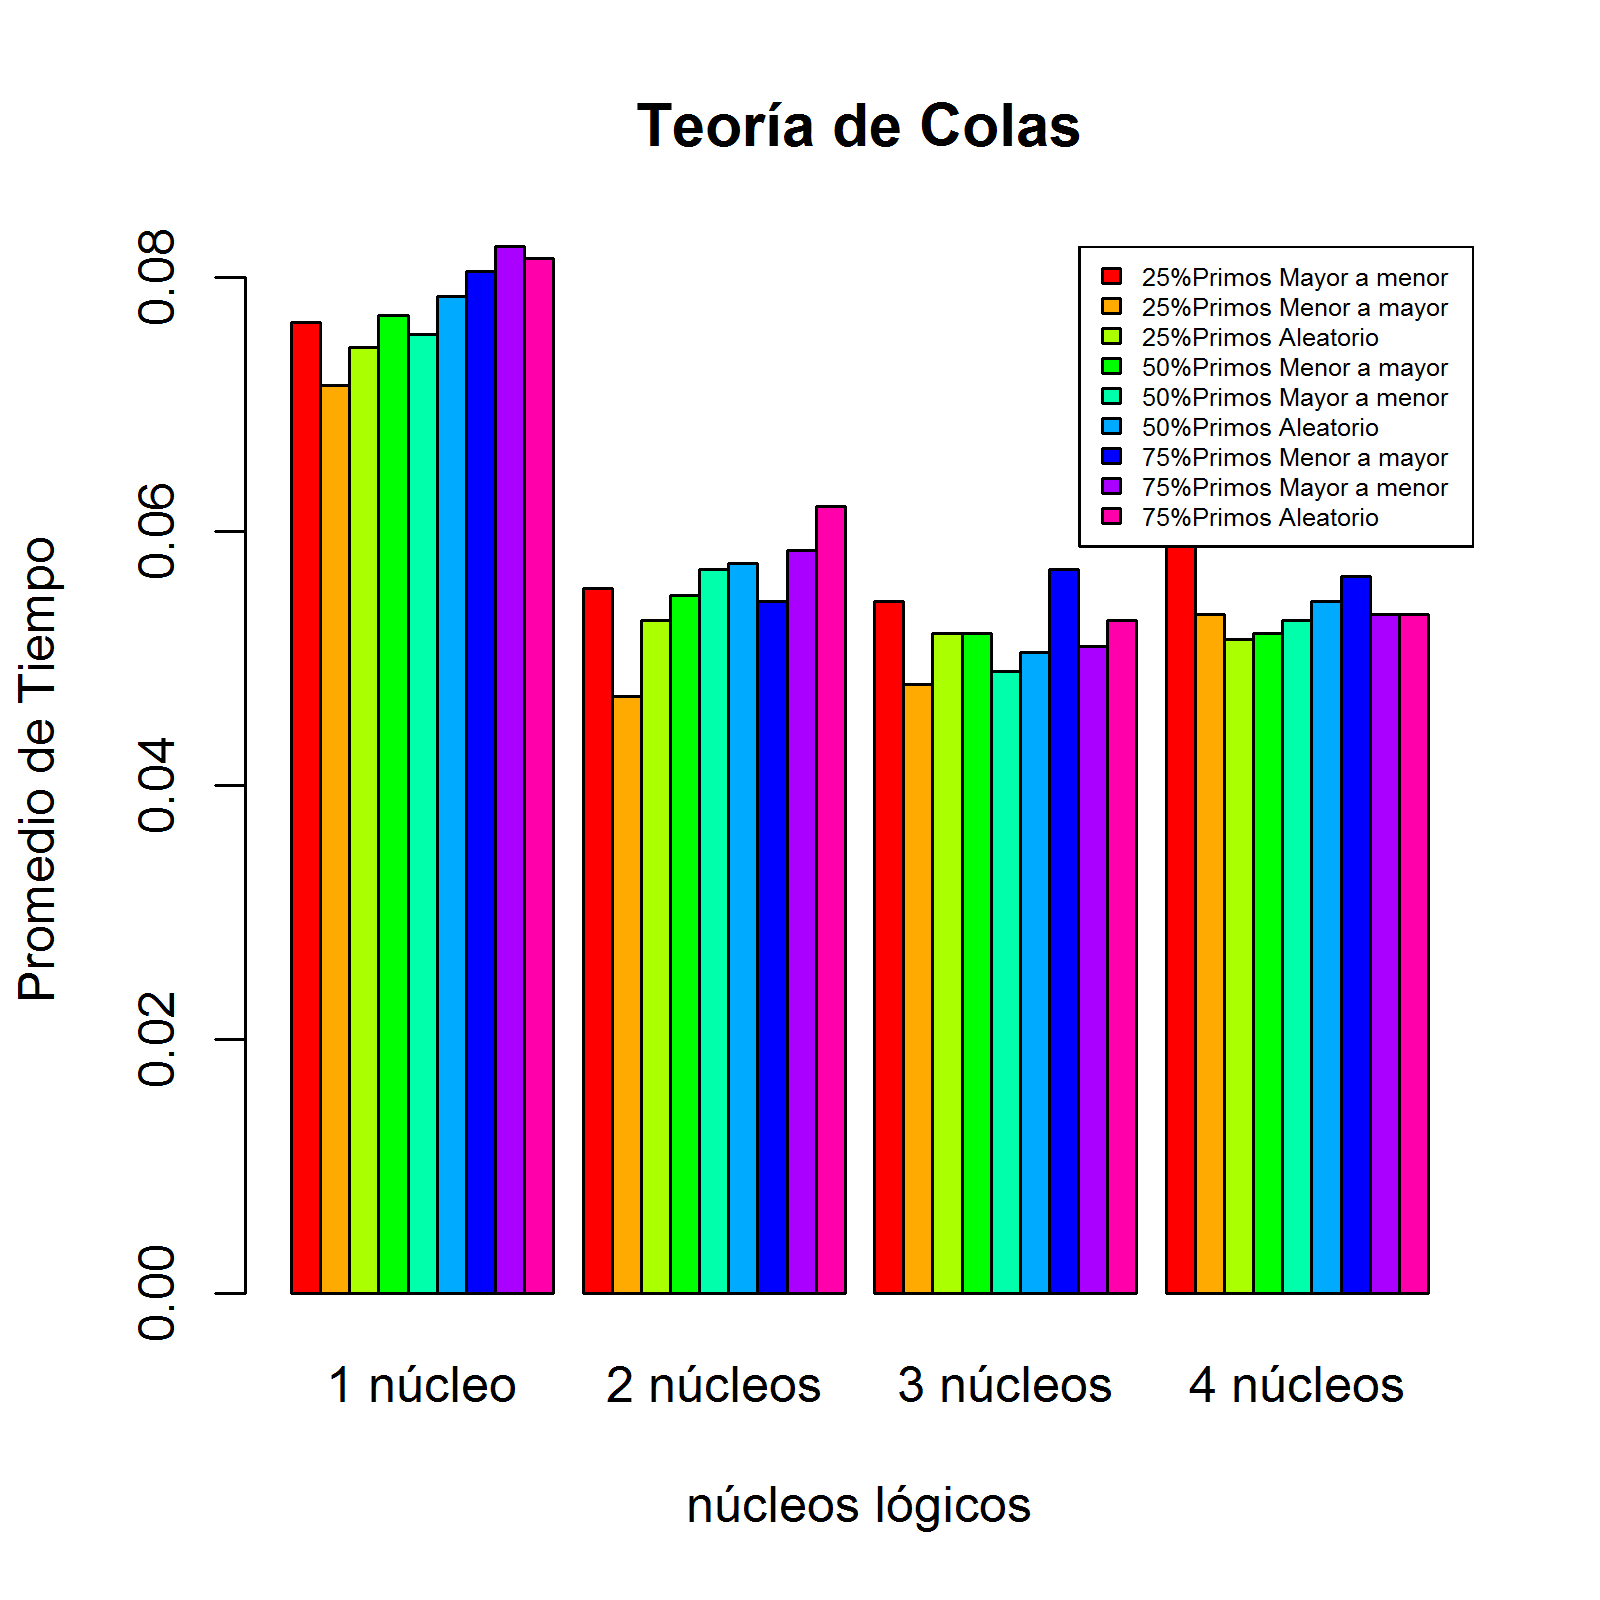
\includegraphics[width=10cm]{teoria_de_colas.png}
\caption{Gráfica de tiempos con variaciones de tipos de datos y núcleos asignados}
\end{figure}


\section{Conclusiones}
En base a los datos obtenidos se puede notar una tendencia a aumentar el tiempo de procesamiento en un vector de datos con más numeros primos, analizados de mayor a menor y utilizando menos núcleos para la tarea.









\bibliographystyle{plainnat}
\bibliography{refe3}
\end{document}